\documentclass[11pt, oneside, a4paper]{scrreprt}
\pagestyle{headings}

\usepackage[german, english]{babel}	% 
\usepackage{robocup} 				% Color ifablue for captions
\usepackage{graphicx}				%  \includegraphics
\usepackage[framed]{mcode}			% MATLAB-Code
\usepackage{pst-all,pst-circ}			% PS-Tricks, Electrical circuits
\usepackage{microtype}
%\usepackage{amssymb}
%\usepackage{graphics}
%\usepackage{multicol}
%\usepackage{alltt}

%\usepackage{epsfig}
%\usepackage{amsmath}
%\usepackage{verbatim}

%\usepackage[official]{eurosym}
\usepackage{scrpage2}
%\usepackage{pdfpages}					% Nicht Brauchbar mit PS-Tricks





% -  -  -  -  -  -  -  -  -  -  -  -  -  -  -  -  -  -  -  -  -  -  -  -  -  -  -  -  -  -  -  -  -  -  -  -  -  -  -  -  -  -  -  -  -  -  -  -  -  -  -  -  - %
\begin{document}
	\begin{titlepage}
\begin{center}

\begin{figure}[!ht]
\begin{center}
\centerline{ 
\includegraphics[height=16mm]{./Pictures/ethz_logo}
              \hspace{25mm}
%              \includegraphics[height=12mm]{psl_plain}}
	    
\includegraphics[height=12mm]{./Pictures/ifalogo_color}}
\end{center}
\end{figure}

\vspace*{20mm}

{Fabio Marti},
{Matthias Roggo},
{David Lehnen},
{Daniel Gilgen}\\

\vspace{10mm} {\LARGE \bf Robocup: Cooperative estimation and prediction of player and ball movement \\} \vspace{10mm}
{Group Project} \\

\vspace{50mm}

Department: \\
IfA -- Automatic Control Laboratory, ETH Z\"urich \\

\vspace{5mm}
Supervising Professor: \\
Prof.~Dr.~John Lygeros, ETH Z\"urich \\

\vspace{5mm}
Supervisor: \\
M.S., Ph.D. Student Sean Summer, ETH Z\"urich \\

\vspace{10mm}
Z\"urich, March 2012

\end{center}
\end{titlepage}
   						% includes title page.tex
	
\section*{Abstract\markboth{ABSTRACT}{ABSTRACT}} % *: Keine Nummerierung des Abschnitts, \markboth: was
% in der Kopfzeile stehen soll

Reliable estimation and prediction are important components for the ETHZ RoboCup Team to win the annual world cup of the Standard Nao Platform League in near future. This paper presents the most important ideas and results of our Group Work in estimation and prediction of a robot soccer match on the Standard Nao Platform. In a first part the simulation of robot and ball movements and the underlying implementation in MATLAB are described and discussed. The second part provides a short theoretical insight in Kalman-filtering and the application of this theory in the framework of the simulation. The last part of this work deals with the multiplicity of measurements and the need of sensor fusion which comes along with this. This Group Work claims to provide a good basis for further investigations in the area of estimation such as improvements in Kalman filtering or sensor fusion and the migration of the implementation on the Nao Platform. 
      					% includes abstract.tex
	\tableofcontents        											% generates the table of content
	\newpage
	\listoffigures													% generates the table of figures
	
	% including Sections
	
%-----Chapter 1: Introduction-------%
\chapter{Introduction}
RoboCup ("Robot Soccer World Cup") is an international ongoing robotics competition founded in 1997.The official goal of the project: "By mid-21st century, a team of fully autonomous humanoid robot soccer players shall win the soccer game, complying with the official rule of the FIFA, against the winner of the most recent World Cup." \cite{wwwRoboCup}
There are a lot of topics of automation and control contained in this project. One topic is the topic of estimation, 
	
%-----Chapter 2: Simulation-------%
\chapter{Simulation}

\section{Playing Field, Robots and Ball}

\section{Random Simulation}


	% -  -  -  -  -  -  -  -  -  -  -  -  -  -  -  -  -  -  -  -  -  -  -  -  -  -  -  -  -  -  -  -  -  -  -  -  -  -  -  -  -  -  -  -  -  -  -  -  -  -  -  -  - %
%-----Chapter 3: Kalman Filtering-------%
\chapter{Theoretical Basics of Kalman Filtering}

\section{Linear Kalman Filter}
There exists a recursive Kalman filter algorithm for discrete time systems.\cite{IntroKF} This ongoing Kalman filter cycle can be divided into two groups of equations
\newline
\begin{enumerate}
	\item Time update equations
	\begin{eqnarray}\label{TupEq}
		%\begin{aligned}
    			\hat{x}_{k}^{-} &= A\hat{x}_{k-1}+Bu_{k-1} \\
    			P_{k}^{-} &= AP_{k-1}A^{T}+Q
  		%\end{aligned}
	\end{eqnarray}
	\item Measurement update equations
	\begin{eqnarray}\label{MupEq}
		%\begin{aligned}
    			K_{k} &= P_{k}^{-}H^{T}(HP_{k}^{-}H^{T}+R)^{-1} \\
    			\hat{x}_{k} &= \hat{x}_{k-1}^{-}+K_{k}(z_{k}-H\hat{x}_{k}^{-}) \\
			P_{k} &= (I-K_{k}H)P_{k}^{-}
  		%\end{aligned}
	\end{eqnarray}
\end{enumerate}

To test this algorithm and to learn something about applying the Kalman filter on linear systems we created an example. A detailed description of the following example can be found in appendix \ref{ExampleKF}. \newline 
We consider a linear, timeinvariant model, given by the following circuit diagram in figure \ref{KFcircuit}.
\begin{figure}[htbp]
	\centering
	\begin{pspicture}(-3,-1)(9,5)
		%nodes
			\pnode(-2,4){A}		\pnode(-2,0){B}		\pnode(8,4){C0}		\pnode(8,0){D}
			\pnode(3,4){A2}		\pnode(3,2){M}		\pnode(3,0){B2}	\pnode(6,4){C2}
			\pnode(6,0){D2}
		%elements
			\coil[intensitylabel=$i_L$,labeloffset=-0.2](A)(A2){$L$}
			\capacitor[tensionlabel=$U_1$,tensionlabeloffset=-1.2,tensionoffset=-0.8,%
					intensitylabel=$i_1$](A2)(M){$C_1$}
			\resistor[tensionlabel=$U_R$,tensionlabeloffset=-1.2,tensionoffset=-0.8](M)(B2){$R$}
			\capacitor[tensionlabel=$U_2$,tensionlabeloffset=-1.2,tensionoffset=-0.8,%
					intensitylabel=$i_2$](C2)(D2){$C_2$}
		%wires
			\wire(B)(D)		\wire(A2)(C0)
			\pscircle[fillstyle=solid](A){0.075}
			\pscircle[fillstyle=solid](B){0.075}
			\pscircle[fillstyle=solid](C0){0.075}
			\pscircle[fillstyle=solid](D){0.075}
		%tension
			\tension(A)(B){$U_{in}$}
			\tension(C0)(D){$U_{out}$}
	\end{pspicture}
    	%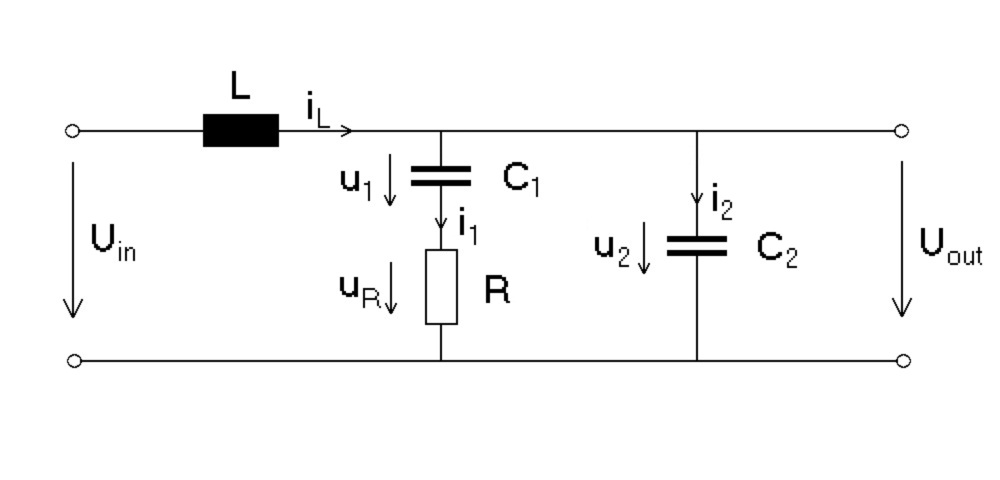
\includegraphics[width=12cm]{./3_KalmanFilter/circuit_diagram.jpg}
  	\caption{Example: Linear electrical circuit.}
  	\label{KFcircuit}
\end{figure}
First we added process noise and measurement noise to the system output. The aim is to get an estimation of the noisy output. Therefore we applied the Kalman filter algorithm based on the equations \ref{TupEq}. In the figure \ref{KFchart}, above we can see the input signal and the ideal measurement of the output signal. That ideal measurement includes process noise, which can obviously not be filtered by the Kalman filtering algorithm. Below one can see the noisy measurement on the left side and the filtered output on the right side.
\begin{figure}[htbp]
	\centering
    	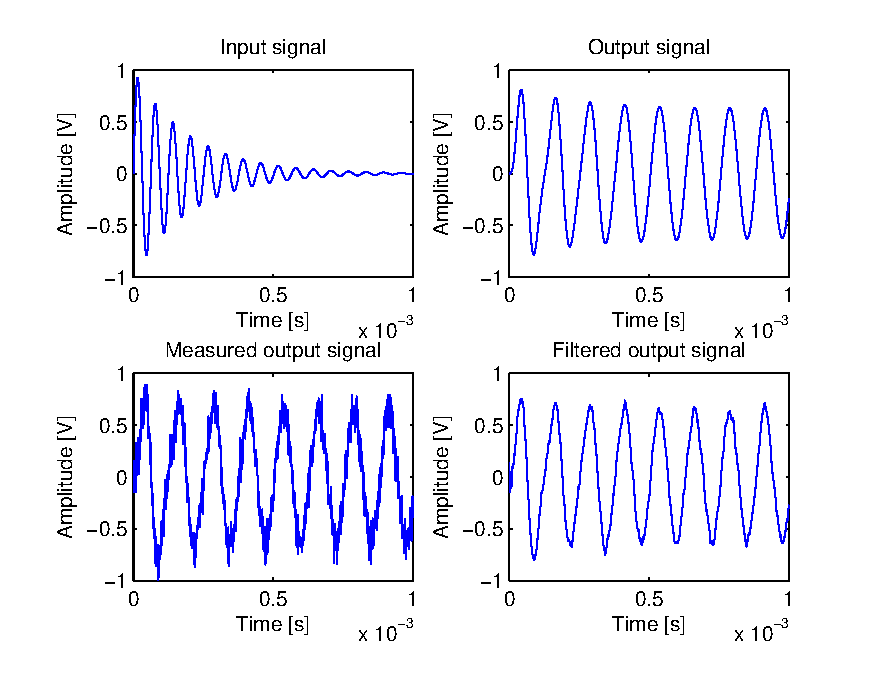
\includegraphics[width=12cm]{./3_KalmanFilterTheory/KFchart.eps}
  	\caption{Example: Input signal, output signal, noisy output, and filtered output.}
  	\label{KFchart}
\end{figure}

\section{Extended Kalman Filter (EKF)}

In the section above we discussed the usage of a Kalman filter on linear systems. Most systems, including the motion equations of our robots, however are nonlinear. Nevertheless linearizing our system around the current estimate still makes our Kalman filter useful and leads to the concept of the extended Kalman filter \cite{IntroKF}. The recursive equations are quite similar to those of the linear Kalman filter
\newline
\begin{enumerate}
	\item Time update equations
	\begin{eqnarray}\label{TupEqEKF}
    			\hat{x}_{k}^- &=& f(\hat{x}_{k-1},u_{k-1},0) \\
    			P_{k}^{-} &=& A_kP_{k-1}A_k^T+W_k Q_{k-1} W_k^T
	\end{eqnarray}
	\item Measurement update equations
	\begin{eqnarray}\label{MupEqEKF}
	%	\begin{aligned}
    			K_{k} &=& P_{k}^- H_k^T(H_k P_k^- H_k^T+V_k R_k V_k^T)^{-1} \\
    			\hat{x}_k &=& \hat{x}_{k-1}^- + K_{k}(z_k - h(\hat{x}_k^-, 0)) \\
			P_k &=& (I-K_k H_k)P_k^-
  	%	\end{aligned}
	\end{eqnarray}
\end{enumerate}

The function \(f(\hat{x}_k,u_k,w_k)\) contains the system's nonlinear dynamics where \(w_k\) represents the current process noise and \(h(\hat{x}_k, v_k)\) denotes the nonlinear state-to-output relationship with the measurement noise \(v_k\). Furthermore the matrices \(A_k\), \(H_k\), \(W_k\) and \(V_k\) are linearizations, i.e. partial drivatives, of their respective functions at time step \(k\)
\newline
%\begin{enumerate}
	\begin{eqnarray}\label{Linearizations}
	%	\begin{aligned}
    			A_{i,j}&= \frac{\partial f_i}{\partial x_j}(\hat{x}_{k-1},u_{k-1},0) \\
    			H_{i,j}&= \frac{\partial h_i}{\partial x_j}(\hat{x}_{k-1},u_{k-1},0) \\
			W_{i,j}&= \frac{\partial f_i}{\partial w_j}(\tilde{x}_k,0) \\
			V_{i,j}&= \frac{\partial h_i}{\partial v_j}(\tilde{x}_k,0)
  	%	\end{aligned}
	\end{eqnarray}
%\end{enumerate}

We dropped the fact that all matrices should have a subscript \(k\) and that they are allowed be different at each time step. Again, before applying the theory to our simulation, we created a generic example of a nonlinear system. Further details can be looked up in section \ref{ExampleEKF}. We did essentially the same as we did for the linear system: We simulated the ideal system, then added process and measurement noise and in the last step checked whether we could get rid of our artifically added measurement noise. The results for a sample run on MATLAB are shown in figure \ref{EKFchart} below

\begin{figure}[htbp]
	\centering
    	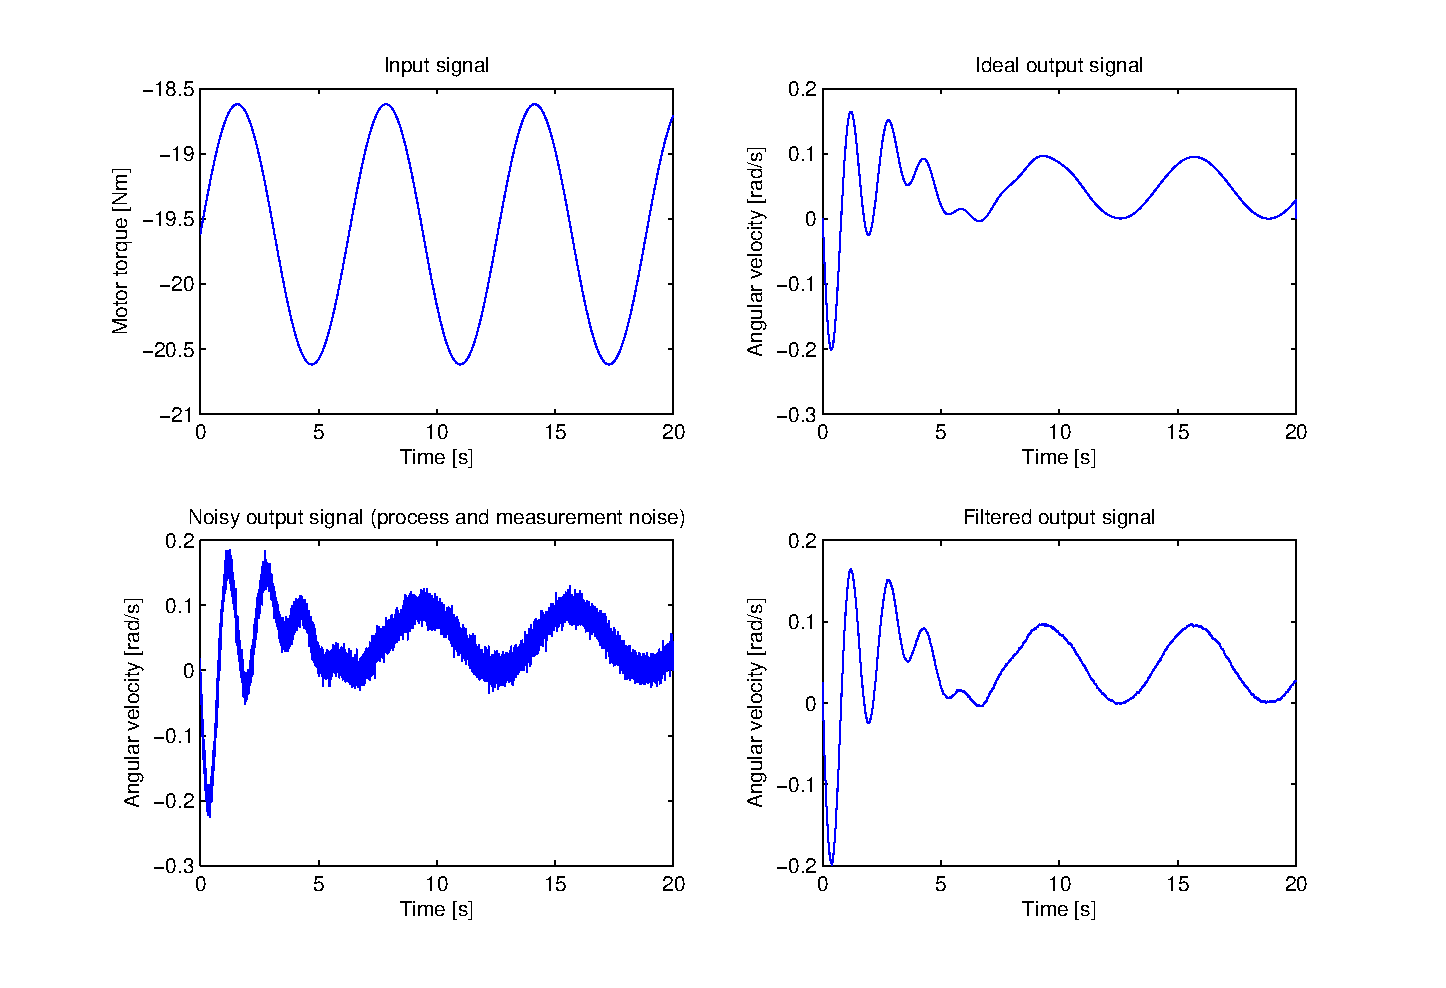
\includegraphics[width=12cm]{./3_KalmanFilterTheory/EKFchart.eps}
  	\caption{Example: Input signal, output signal, noisy output, and filtered output.}
  	\label{EKFchart}
\end{figure}

The two pictures above show the sinusoidal input on the left and the ideal output, i.e. without process and measurement noise, on the right. Thereunder we can see the plots of the noisy signal and the signal after it has been filtered by the extended Kalman filter. We can conclude that the extended Kalman filter too provides an acceptable performance if our measurement noise is not too big.



	
%-----Chapter 4: Estimation-------%
\chapter{Kalman Filtering: Implementation in the MATLAB Environment}

\section{Estimation of the Robots}

As we have seen before, the motion equations of the robots are nonlinear, which makes it necessary to use an extended Kalman filter for the estimation of the robots. The function {\fontfamily{pcr}\selectfont robot\_ekf(robot\_m,robot\_e,m\_values,e\_values,d\_omega,v,P).m} is dedicated for this task. As stated in the theory above, we will need the old estimates and the measurements in order to compute new estimates. Most matrices like the covariance matrices or the Jacobian matrices are the same for all eight robots and hence have to be defined only once. The error covariance \(P\) and the estimator \(K\) on the other side have to be stored for every robot individually, therefore we will use cell arrays for this task. The initialization in MATLAB of these parameters is shown below

\lstinputlisting[firstline=18, lastline=27]{../Simulation/Merge/robot_ekf.m}
\parskip 20pt

In a next step we calculate the Kalman estimate for every robot. In a former version of the function, the two cell arrays {\fontfamily{pcr}\selectfont m\_values} and {\fontfamily{pcr}\selectfont e\_values} contained a history of the last measurements and estimates of the robots. They were used to improve the performance of the extended Kalman filter. The collision detection of former versions of the simulation made it necessary for the filter algorithm to be responsive to large changes of the direction of the robots. Since the Kalman filter itself couldn't handle these rapid changes, we needed a function that indicates that the measurements are much more reliable if there is a huge difference between them and the estimates over a certain space of time. The essential functionality was  to reduce the matrix \(R\), which caused the extended Kalman filter to heaviliy trust the incoming measurements. For this task a history of former measurements and estimates was necessary. But since these problems disappeared with the introduction of collision avoidance, the used methods are obsolete. The function {\fontfamily{pcr}\selectfont i\_measurement(robot\_m,m\_values,e\_values).m} however is still needed for another reason: Measurement drops over a large time span will cause divergence between estimated values and actual values. Regaining visual information from robots will eventually lead to convergence of both values, but this usually happens way too slow. Therefore we needed a method to get the estimates back on track, if there is a huge difference between them and the measurements. The following computations are done for every robot

\lstinputlisting[firstline=32, lastline=37]{../Simulation/Merge/i_measurement.m}

The current implementation uses probabilistic methods, to decide how to reduce the matrix \(R\). The key idea behind this method is, to compute how probable it is, that the measurements and estimates differ even more, than they actually do. For example: If the estimation of a variable is equal to its measurement, we have probability \(100\%\) that their difference is even bigger. In this case \(R\) is multiplied by 1; there is no need to trust the measurement more than usual because our estimation is pretty good.
Another challenge of the estimation was how to get information about the inputs of enemy robots. This task is done by {\fontfamily{pcr}\selectfont input\_approximation(robot\_m,m\_values,v).m}. The goal is to reconstruct the change of the angular position and the velocity only by looking at the measurements. Since the change of the angular position is a random process which produces statistically independent values for every timestep, a prediction of this value is impossible. The best one can do is therefore to form the difference between the robot's measured direction in time step \(k\) and \(k-1\). The input variable will now contain some error, but this can be handled by the Kalman filter as long as the error is small enough. For the velocity on the other side we use a different method. The velocity is computed out of the position measurements, which are heavily affected by noise. Therefore the computation of the velocity in only one timestep is not very reliable. We solved this problem by using a sliding window, meaning that the velocity, we use as an input, is the mean value of velocities of several timesteps. This is a valid approach, since contrary to the change of angular position, the velocity can't change very rapidly. The corresponding code excerpt is shown below

\lstinputlisting[firstline=33, lastline=35]{../Simulation/Merge/input_approximation.m}

If there are no measurements at all, we assume maximal velocity and zero change in direction.
After facing the problems presented above, we could implement the time update and measurement update equations just as they were stated in the theory. The MATLAB-code below forms the core of the extended Kalman filter for the robots

\lstinputlisting[firstline=65, lastline=79]{../Simulation/Merge/robot_ekf.m}
\parskip 20pt

The prediction of the robot's position and direction can be done for every time step, but the correction is only possible if all measurements are available. This is not the case for example if robots don't get visual information of other robots. With the if-statement we accomodate this fact. So the typical Kalman cycle is only executed if we have measurement on the positions and the direction. Otherwise we drop the measurement update, i.e. our new estimate is simply a simulation of the robot's motion with the former estimates.
\parskip 10pt


\section{Estimation of the Ball}

The estimation of the ball is done by {\fontfamily{pcr}\selectfont ball\_kf(Ball\_oe, Ball\_m, P\_oe).m}. This function has essentially the same functionality as the Kalman filter for the robots. If there are measurements of the ball's position and direction, the time update and measurement update equations are computed, otherwise only the time update equations are calculated. The only difference between the ball and the robots is, that large changes of its motion are possible. Such discrete events are handled with the if-statement shown below

\lstinputlisting[firstline=23, lastline=28]{../Simulation/Merge/ball_kf.m}

So the Kalman filter for the ball is switch triggered: If a certain threshold of acceptable error in position or direction estimation is exceeded, we reset the Kalman filter. This has the effect that the tracking of the ball is quickly reestablished after a collision with a robot or with some of the boundaries.




	
%-----Chapter 5: SensorFusion-------%
\chapter{Sensor Fusion}
In RoboCup every robot works autonomous except a WLAN connection between the teammates. So the whole team can share information to optimize their game.
Through his field of view every robot can bring in some informations about the playing field, other robots and about the ball. Now to optimize the estimation and to exploit the informations from the robots, the team can share this informations in form of a sensor fusion algorithm.
Sensor fusion offers a great opportunity to overcome physical limitations of sensing systems.\cite{IntroSF} 

In the case of RoboCup we need as so called High-level fusion (decision fusion). Methods of decision fusion do not include only the combination of position, edges, corners or lines into a feature map. Rather they imply voting and statistical methods. \cite{IntroSF}. 


\section{Sensors of the Robots}
The robots come with a camera with a defined field of view. There are no other sensors or informations which can be used for estimation of the positions. 
There are three types of sensor configuration regarding to sensor fusion. \cite{IntroSF}
\begin{itemize}
	\item Complementary
	\item Competitive
	\item Cooperative
\end{itemize}
In the RoboCup case all the types can occur. The sensor configuration is complementary if a region is  observed by only one robot or camera. And if there are two or more cameras the sensor configuration can be competitive or cooperative.


\section{Mathematical model for Sensor Fusion}

We have chosen a situation-based statistical model for our purposes. The covariance of a measurement depends on the situation at which a robot gains the positon and the angle of another robot. Differently said: There are several scenarios under which a robot can get visual information and each scenario is characterized by the quality of a measurement, implying the value of the covariance. In our case, the measurement of the \(i\)-th robot looks as follows

\begin{enumerate}
	\begin{eqnarray}\label{measurement}
    			\hat{X}_{i} &=& X + w_i
	\end{eqnarray}
\end{enumerate}

\(X\) is the deterministic variable we want to know (i.e. position or direction) and \(w_i\) is white Gaussian noise with a certain covariance \(\sigma_i^2\), depending on the condition under which a robot got the information, so \(w_i \tilde \mathcal{N}(0,\sigma_i^2)\). A fusion of \(n\) measurements now looks as follows

\begin{enumerate}
	\begin{eqnarray}\label{fusion}
    			 Y &=& a_1 \hat{X}_{1} + a_2 \hat{X}_{2} + \ldots + a_n \hat{X}_{n}
	\end{eqnarray}
\end{enumerate}

where \(n\) in our case can be at most 4. The main task of sensor fusion is to find the weights \(a_i\). To find them, we make two reasonable assumptions: The mean of the fused measurement has to be equal to \(X\). On the other side the mean of the squared error has to be minimal. Formally we want

\begin{enumerate}
	\begin{eqnarray}\label{assumptions}
    			 E[Y] = X \qquad  &\mathrm{and}& \qquad E\left[ (Y-X)^2 \right] \rightarrow 						\mathrm{minimal} 
	\end{eqnarray}
\end{enumerate}

The first condition leads to the simple fact, that all weights have to sum up to \(1\)

\begin{enumerate}
	\begin{eqnarray}\label{side_condition}
    			 a_1 + \ldots + a_n = 1 \qquad &\Longleftrightarrow& \qquad G(a_1, \ldots, a_n) = a_1 +   				\ldots a_n - 1
	\end{eqnarray}
\end{enumerate}

For the second condition, we are assuming that all \(w_i\) are mutually independent, so we have \(E[w_i w_j] = 0, \; i \neq j\). Taking (\ref{side_condition}) into account leads to the second condition

\begin{enumerate}
	\begin{eqnarray}\label{main_condition}
    			 F(a_1,\ldots,a_n) = a_1^2\sigma_1^2 + \ldots + a_n^2 \sigma_n^2 &\rightarrow&  					\mathrm{minimal}
	\end{eqnarray}
\end{enumerate}

The generic approach is now to solve equation (\ref{main_condition}) with \(\nabla F(a_1,\ldots,a_n) = 0\). This attempt fails, because we also have to meet the side condition from equation (\ref{side_condition}). Therefore we use the method of Lagrange multipliers \cite{Blatter}. The equations we have to solve, are shown below

\begin{enumerate}
	\begin{eqnarray}\label{lagrange_multipliers}
    			 \nabla F(a_1,\ldots,a_n) = \lambda \nabla G(a_1,\ldots,a_n), \qquad && \qquad G(a_1,\ldots,a_n) = 0
	\end{eqnarray}
\end{enumerate}

The system of equations above consists of \(n+1\) equations and \(n+1\) unknowns, so there is a unique solution which is shown below

\begin{enumerate}
	\begin{eqnarray}\label{solution}
    			 a_i &=& \frac{\sigma_i^{-2}}{\sum_{j=1}^n \sigma_j^{-2}}
	\end{eqnarray}
\end{enumerate}

In a final step, we are interested in the statistical properties of our fused measurement. The mean is already given by condition (\ref{assumptions}). Since \(Y\) is a Gaussian random variable we only need the covariance \(\sigma_Y^2\) to fully describe \(Y\). We get

\begin{enumerate}
	\begin{eqnarray}\label{solution}
    			 \sigma_Y^2 = E\left[ Y^2 \right] - E[Y]^2 &=& \frac{1}{\sum_{j=1}^n \sigma_j^{-2}}
	\end{eqnarray}
\end{enumerate}

A short analysis reveals, that \(\sigma_Y^2 < \sigma_i^2, \; \forall i\); the covariance of the fused measurement is smaller than the covariance of every single measurement. Or in other words: The fused measurement is, from a statistical point of view, always more precise than the measurement of only one robot, even if we fuse a very good and a very bad measurement.


\section{The implementation in MATLAB}


	
%-----Chapter 6: FlawsOutlook-------%
\chapter{Flaws and Outlook}

Several problems which can occur in a real Nao soccer match are covered by our design of the model such as measurement drops, measurement fusion or the fact that inputs of the opposing team are unknown. However there are still practical challenges which we do not encounter in our work. Maybe the most important challenge is the provision of measurements and their related covariances. Up to this point we simply assumed that there is an algorithm which computes the positions and directions of objects on the playing field. We didn't care about the fact whether this can be done in a reliable way or within a reasonable space of time. This task was beyond the scope of this work and certainly could be the subject of another whole group work for the people in the ETHZ RoboCup Team which are occupied with perception.
\parskip 0pt

Other problems arise from the restrictions of our chosen model, for example the assumption that there are only three scenarios under which measurements are gathered. In reality we are probably faced with much more possibilities, that do not only depend on whether a robot sees a landmark or not but also on the actual sight distance to an object or the head angle of a robot. Furthermore the measurement noise may be coloured and not white, so our model would be inaccurate in describing the uncertainty in the given system. Those kind of issues can be summarized as ''lack of detail'', the approximation to reality is not close enough. This can be solved by a better and deeper analysis of the system.

Last but not least there are still several things, that were only partly or not at all considered in our work and which have huge potential for the further localization task. One main aspect here is certainly the practical application of the simulation on the Nao Platform. Not only that it is of course the main goal to have a working estimation and prediction for a real Nao soccer match but also that further improvements of the estimation algorithms will only be possible if they are tested in real environment with real constraints. The modularity of our simulation allows improvements in specific areas concerning estimation. For example the tracking of the ball may be improved too by replacing the extended Kalman filter by a so called particle filter, so switching from deterministic to probabilistic methods. It is also imaginable to have hybrid forms like it is partly done for the extended Kalman filter of the robots (see Ch. 4.1). As a third point one could mention the vast improvements which are possible in estimation if the robots are not acting randomly but if they have a strategy that governs their movements. In terms of localization that would mean that blue robots actively seek getting good measurements and that for example losing the current position of the ball for long periods is not possible anymore. More extensions of the current basic configuration such as better input approximation of enemy robots, the prediction of enemy movements or better handling of discrete events are also thinkable and can have positive effects on the overall performance.



	
%-----Appendix-------%
\appendix               	% at this point the appendix starts
\chapter{Examples} 
\section{Kalman Filtering of Linear System} \label{ExampleKF} 
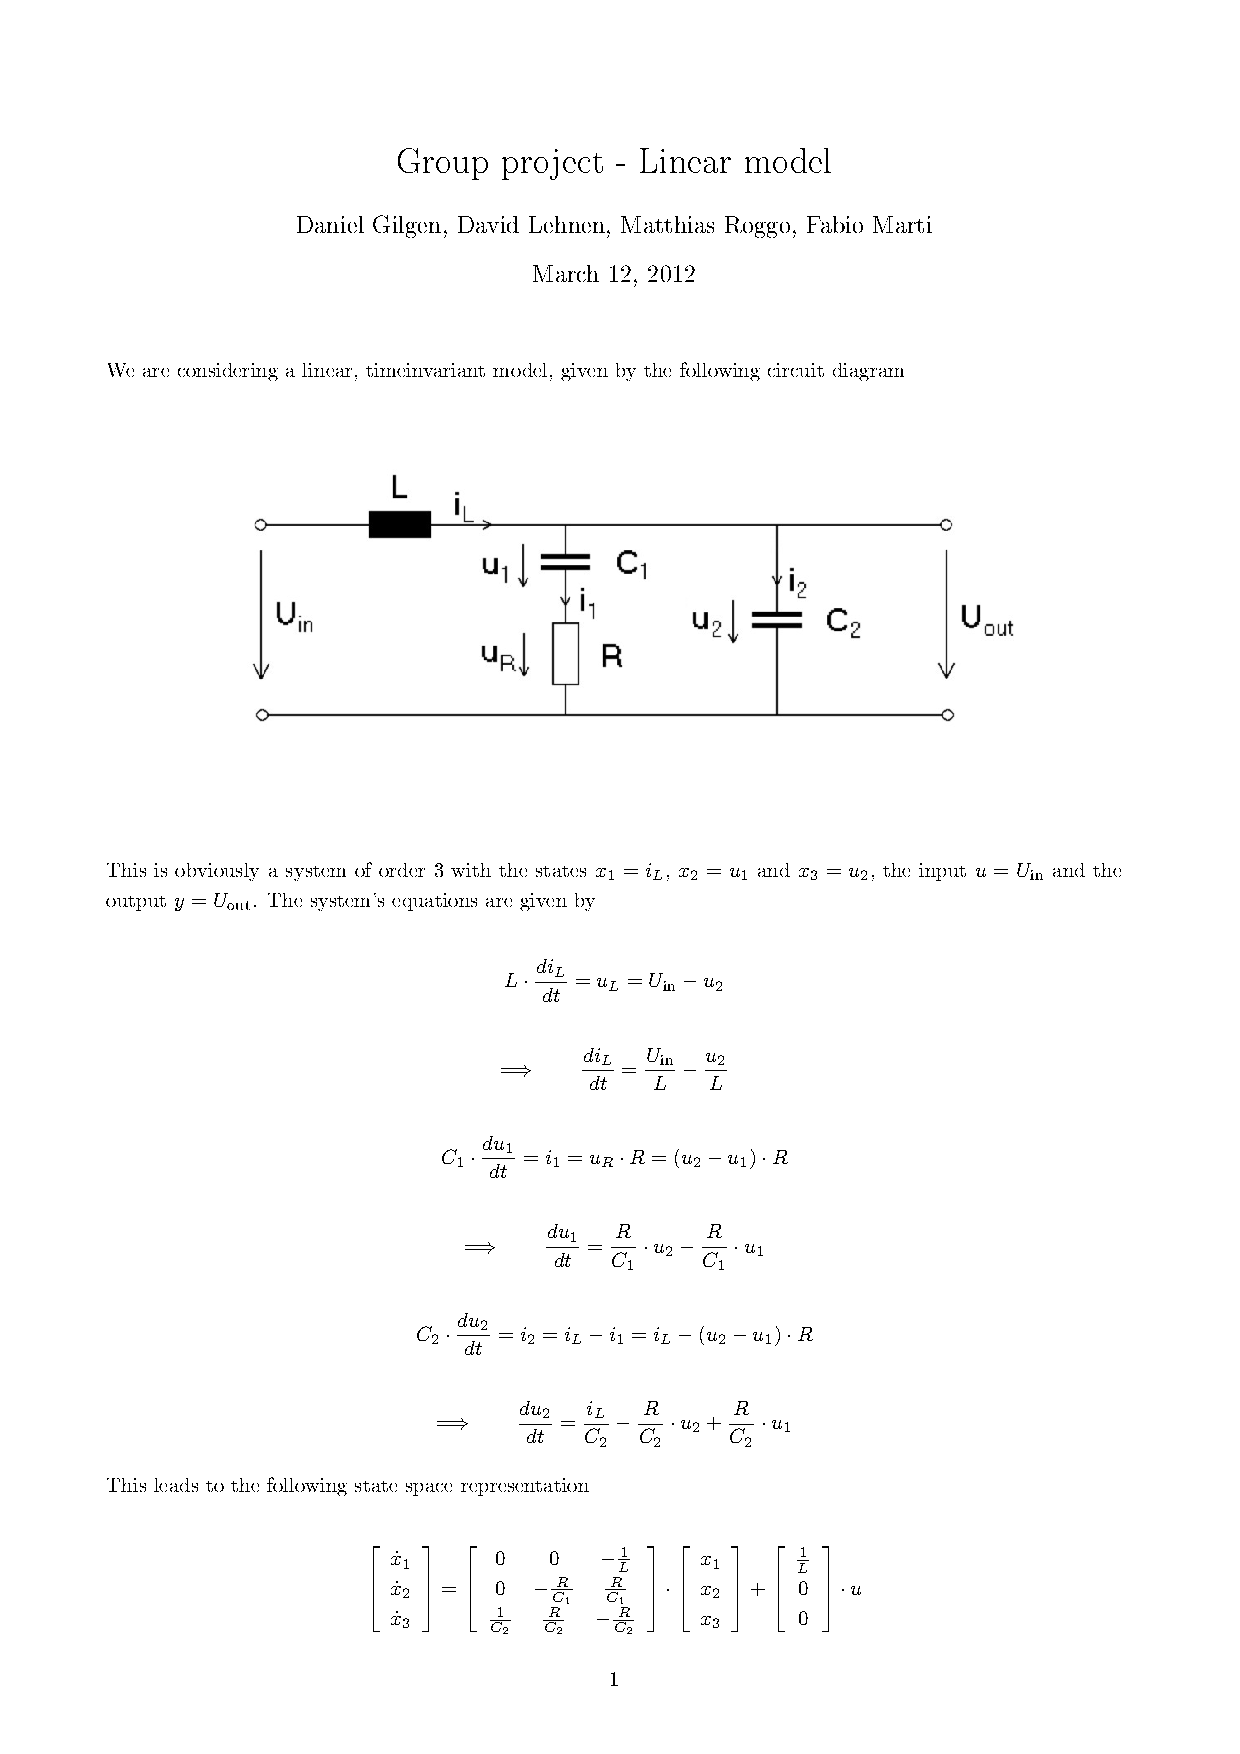
\includepdf[pages=-]{./appendix/linear_model.pdf}

\section{Kalman Filtering of Nonlinear System} \label{ExampleEKF} 
	
% Literaturverzeichnis

\addcontentsline{toc}{section}{Literatur}
\begin{thebibliography}{30}

%{\Large\textbf{Books and Articles}}

\bibitem{IntroKF} G. Welch and G. Bishop, ``An Introduction to the Kalman Filter,'' UNC-Chapel Hill, 2006.

\bibitem{RulesRC} RoboCup Technical Committee, ``RoboCup Standard Platform League (Nao) Rule Book,'' RoboCup, 2011.

\bibitem{wwwRoboCup} \texttt{http://www.robocup.org/about-robocup/objective/}\\
Webpage of the RoboCup Organisation, last access:
08.05.2012

\bibitem{IntroSF} Wilfried Elmenreich, ``An Introduction to Sensor Fusion,'' Institut für Technische Informatik Vienna University of Technology, 2001.

\bibitem{Blatter} Christian Blatter, ``Ingenieur Analysis 1 und 2,'' Springer, 1996.


\end{thebibliography}
    											% includes title literature.tex
\end{document}
